\documentclass[aspectratio=169,11pt]{beamer}
\usepackage{fontspec}
\setsansfont[Extension=.otf,UprightFont=*-regular,BoldFont=*-bold,ItalicFont=*-italic,BoldItalicFont=*-bolditalic]{texgyreheros}
\usepackage{booktabs}
\usepackage{pgfplots}
\pgfplotsset{compat=1.18}

\definecolor{Ocean}{HTML}{0C2D3B}
\definecolor{Teal}{HTML}{007870}
\definecolor{Rust}{HTML}{A5412B}
\definecolor{Slate}{HTML}{48616A}
\definecolor{Paper}{HTML}{F5F7F6}
\setbeamercolor{normal text}{fg=Ocean,bg=Paper}
\setbeamercolor{structure}{fg=Teal}
\setbeamercolor{frametitle}{fg=Ocean}
\setbeamerfont{frametitle}{size=\Large,series=\bfseries}
\setbeamertemplate{navigation symbols}{}
\setbeamersize{text margin left=9mm,text margin right=9mm}
\setbeamertemplate{frametitle}{%
  \vspace{5mm}\insertframetitle\par\vspace{3mm}%
}

\newcommand{\labeltext}[1]{\textcolor{Teal}{\textbf{#1}}}
\newcommand{\details}[1]{{\small\color{Slate}#1}}
\newcommand{\metric}[1]{{\LARGE\bfseries\color{Teal}#1}}

\begin{document}

{
\setbeamercolor{background canvas}{bg=Ocean}
\setbeamercolor{normal text}{fg=white}
\begin{frame}[plain,c]
  \color{white}
  {\small\bfseries ESILV · PROGRAMMING IN DATA SCIENCE · DIA3\par}
  \vspace{7mm}
  {\Huge\bfseries Global shark attacks\par}
  \vspace{2mm}
  {\large Where and when are shark incidents reported?\par}
  \vspace{10mm}
  Maxime Laurent · Louis Le Forestier\\
  Baptiste Noailhac · Romain Thepaut\par
  \vspace{3mm}
  {\small Global Shark Attack File and World Bank tourism arrivals}
\end{frame}
}

\begin{frame}[t]{From raw records to 4,033 incidents}
  \begin{columns}[T,onlytextwidth]
    \begin{column}{.43\textwidth}
      \metric{25,723}\par
      \details{Raw CSV rows, including blank padding}\par
      \vspace{5mm}
      \metric{4,033}\par
      \details{Incidents retained for 1960–2018}\par
    \end{column}
    \begin{column}{.55\textwidth}
      \labeltext{Time}\quad Year, month and local season\par
      \medskip
      \labeltext{Place}\quad Country and coastal area\par
      \medskip
      \labeltext{Incident}\quad Activity, species and fatality\par
      \vspace{5mm}
      We profiled missing values, removed blank rows and administrative fields, and standardized country and activity names.
    \end{column}
  \end{columns}
  \vspace{5mm}
  \details{Coastal coordinates are assigned by area in the Global Shark Attack File analysis.}
\end{frame}

\begin{frame}[t]{Reported incidents and recurring profiles}
  \begin{columns}[T,onlytextwidth]
    \begin{column}{.51\textwidth}
      \labeltext{Reported incidents by country}\par
      \smallskip
      \begin{tabular}{@{}lr@{}}
        \toprule
        United States & 1,756 \\
        Australia & 704 \\
        South Africa & 432 \\
        \bottomrule
      \end{tabular}\par
      \vspace{4mm}
      \details{Surfing accounts for 1,257 reports. The recorded fatal share is 5.25\%.}
    \end{column}
    \begin{column}{.45\textwidth}
      \labeltext{Apriori and association rules}\par
      \smallskip
      A 3\% minimum support retained 417 frequent itemsets. A lift threshold of 1.05 retained 2,262 rules.\par
      \vspace{4mm}
      \details{Support measures frequency. Confidence gives the conditional share. Lift compares that share with the overall baseline.}
    \end{column}
  \end{columns}
  \vspace{4mm}
  \details{Grouping also reports the share of incidents recorded as fatal, by activity and identified species.}
\end{frame}

\begin{frame}[t]{Seasonal peaks and coastal clusters}
  \begin{columns}[T,onlytextwidth]
    \begin{column}{.58\textwidth}
      \labeltext{Monthly share of reports (\%)}\par
      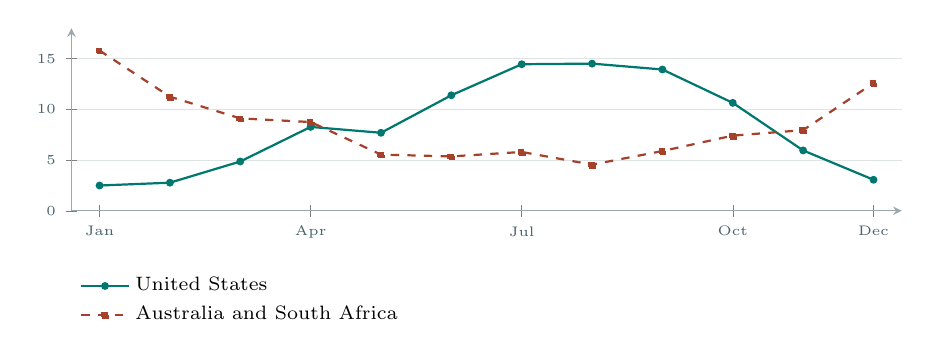
\begin{tikzpicture}
        \begin{axis}[
          width=\linewidth,height=39mm,scale only axis=false,
          xmin=0.6,xmax=12.4,ymin=0,ymax=18,
          xtick={1,4,7,10,12},xticklabels={Jan,Apr,Jul,Oct,Dec},
          ytick={0,5,10,15},tick align=outside,
          tick label style={font=\tiny,text=Slate},
          axis line style={draw=Slate!55},axis lines=left,
          ymajorgrids,grid style={draw=Slate!18},
          legend style={draw=none,fill=none,at={(0,-0.30)},anchor=north west,
            legend columns=1,font=\scriptsize,cells={anchor=west}},
        ]
          \addplot[Teal,thick,mark=*,mark size=1pt] coordinates {
            (1,2.49) (2,2.77) (3,4.86) (4,8.27) (5,7.69) (6,11.39)
            (7,14.45) (8,14.51) (9,13.93) (10,10.64) (11,5.95) (12,3.06)};
          \addlegendentry{United States}
          \addplot[Rust,thick,dashed,mark=square*,mark size=1pt] coordinates {
            (1,15.8) (2,11.25) (3,9.11) (4,8.75) (5,5.54) (6,5.36)
            (7,5.8) (8,4.55) (9,5.89) (10,7.41) (11,7.95) (12,12.59)};
          \addlegendentry{Australia and South Africa}
        \end{axis}
      \end{tikzpicture}
    \end{column}
    \begin{column}{.38\textwidth}
      \labeltext{Five-year forecast}\par
      \smallskip
      \details{Prophet fitted to 1960–2017 projects 112–118 annual reports in 2018–2022, with wide uncertainty.}\par
      \vspace{4mm}
      \labeltext{Spatial clustering}\par
      \smallskip
      \details{95.6\% of reports received coastal coordinates. K-means groups them into six clusters. OPTICS checks local density.}
    \end{column}
  \end{columns}
\end{frame}

\begin{frame}[t]{The ranking changes after accounting for arrivals}
  \labeltext{Matched incident and tourism records, 1995–2018}\par
  \vspace{3mm}
  \begin{tabular}{@{}lrr@{}}
    \toprule
    Country or territory & Reported incidents & Incidents / 1M arrivals \\
    \midrule
    United States & 1,180 & 0.39 \\
    Australia & 433 & 3.14 \\
    New Caledonia & 31 & 18.31 \\
    \bottomrule
  \end{tabular}\par
  \vspace{5mm}
  Across 355 matched country-years, arrivals and incident counts had a Pearson correlation of \(r=0.60\).\par
  \medskip
  \details{The join omits years with no recorded incident and years without tourism data. Arrivals measure tourism volume. The incident records include residents and visitors.}
\end{frame}

\begin{frame}[t]{Dashboard demo}
  \labeltext{See how the pattern changes with the filters}\par
  \medskip
  Filter by year, country and activity to update the counts and coastal map. Open the temporal tab to compare seasonal peaks.\par
  \vspace{6mm}
  \labeltext{Interpret the results in context}\par
  \medskip
  Reports peak in local summer in the studied regions. Reporting coverage, approximate coordinates and missing exposure data limit comparisons.\par
  \vspace{6mm}
  \details{\href{https://github.com/groupe-dia3-ml/programming-for-data-science}{Project repository} · Laurent\_notebook.ipynb · Laurent\_dashboard.html}
\end{frame}

\end{document}
